\documentclass[14pt]{extreport}
\usepackage{gost}
\usepackage{hyperref}
\usepackage{makecell}
\usepackage{ragged2e}
\usepackage{graphicx}%Вставка картинок правильная
\usepackage{float}%"Плавающие" картинки
\usepackage{wrapfig}%Обтекание фигур (таблиц, картинок и прочего)
	
\usepackage{lscape}
\justifying
\makeatletter
\@addtoreset{figure}{part}% Reset figure numbering at every part
\makeatother
\renewcommand{\thefigure}{\arabic{figure}}% Figure number is part.figure
\renewcommand{\thetable}{\arabic{table}}



%Тут можно вставить дополнительные пакеты

\begin{document}
\pagestyle{empty} %  выключаем нумерацию
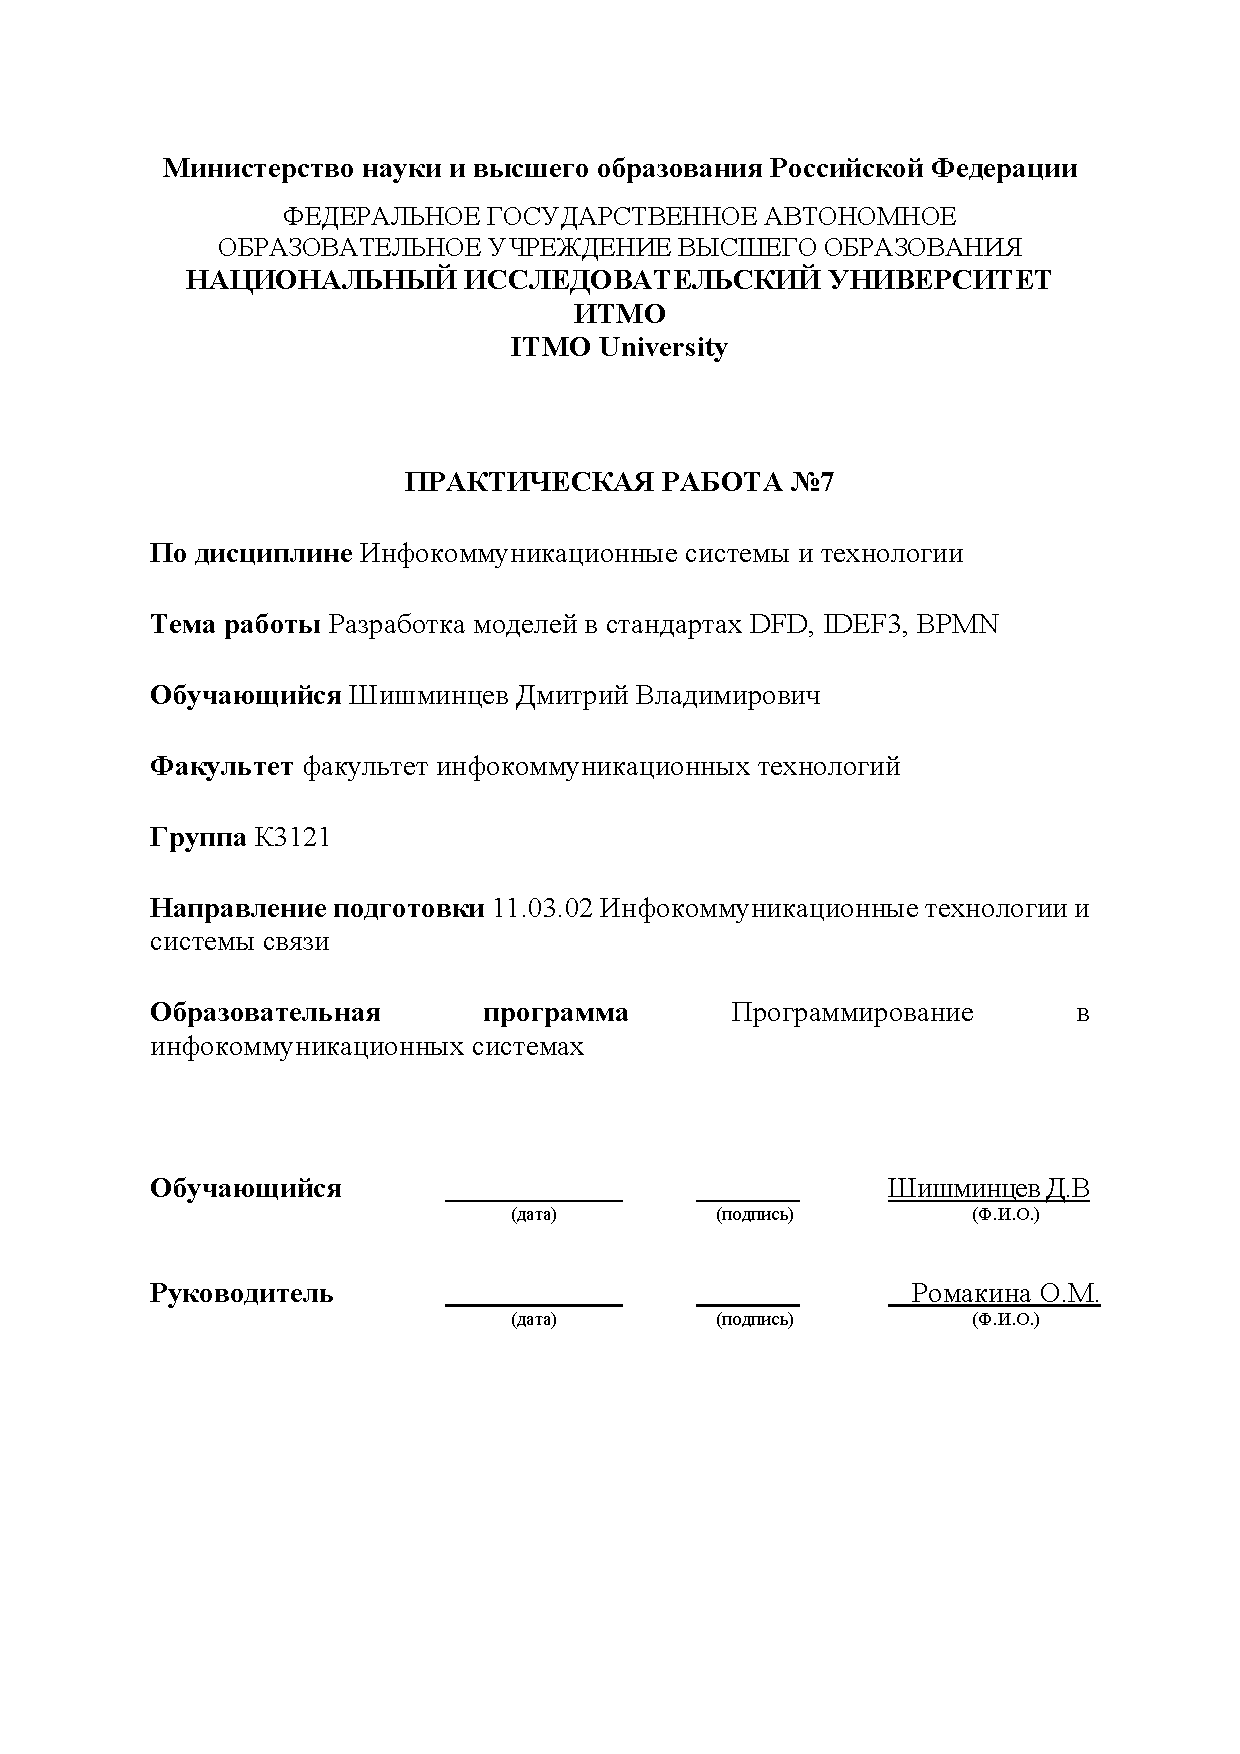
\includepdf[pages=-,pagecommand={}]{title_page.pdf}


\pagestyle{plain} % включаем нумерацию
\tableofcontents
\intro\label{intro} 

Данная практическая работа содержит в себе краткое описание предметной области функционирования и основных пользователей будующей информационной системы, так же модели информационной системы по стандартам DFD, IDEF3, BPMN.


\chapter{ОПИСАНИЕ ИДЕИ ИНФОРМАЦИОННОЙ СИСТЕМЫ \label{chapter1}}

\section{Основной функционал}

Информационная система MEET ME представляет из себя веб-приложение для планирования встреч с друзьями и родственниками в виде календаря. 
Приложение показывает пересечение свободного времени пользователя с одним или несколькими его друзьями.
C помощью данного приложения пользователь может эффективно планировать встречи со своими друзьями, родственниками или знакомыми не тратя огромное количество времени на согласования времени. 

После создания аккаунта, пользователю будет предложено настроить свое расписание. Пользователь выбирает дни и время, когда он имеет возможность для встречи. 
Настроив свое расписание, пользователь должен добавить своих друзей.  Добавление друзей идет посредством отправки запроса другу на его электронную почту указаную при регистрации аккаунта.

Настроив свое расписание и добавив друзей, пользователю начинают отображаться пересечения в расписании с его друзьями в виде календаря. Пользователю не показывается полностью расписание встреч его друзей ради сохранения приватности. Пользователь может отправить приглашение на встречу своему другу если их свободное время пересекается в приложении. Приглашение отобразится у его друга и он сможет принять или отклонить его. Приняв приглашение у обоих пользователей отобразится встреча в их календаре. 

\section{Основные пользователи}

Информационная система будет иметь только прямых конечных пользователей. Система не требует модераторов, менеджеров и прочих пользователей.
Целевая аудитория данной информационной системы достаточно широка. Основными пользователями будут молодые, общительные люди, которые стараются грамотно распределять свое время (ученики старших классов, студенты, работающая молодежь).


\chapter{Модели и диаграммы}
    \section{Модели по стандарту DFD}
        В данном разделе, в качестве дополнения к функциональной модели инфомрационной системы по стандарту IDEF0, представлены диаграммы по стандарту DFD. Для контекстной диаграммы IDEF0 (рисунок \ref{fig:d1}) представлена декомпозиция (рисунок \ref{fig:d2}). Для блоков <<Авторизация>> и <<Определение общего свободного времени>> представлены диаграммы в стандарте DFD (рисунок \ref{fig:d3}, рисунок \ref{fig:d4}).

        \begin{landscape}
            \begin{figure}[h]   
                \centering
                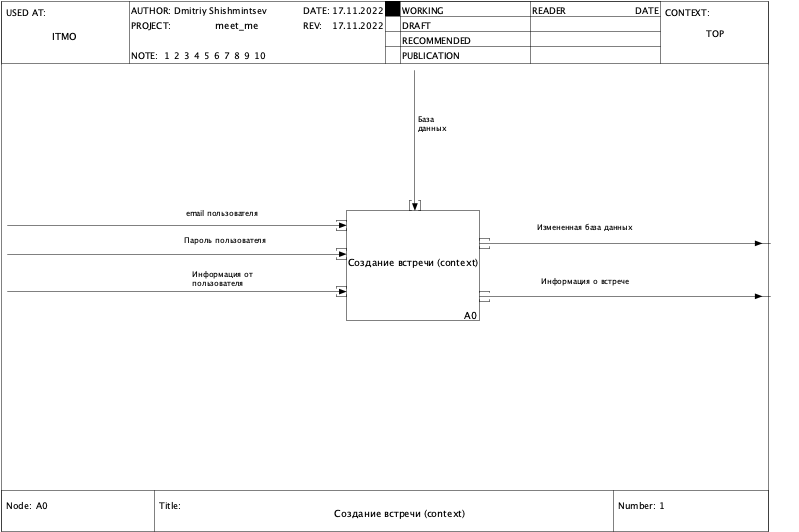
\includegraphics[width=0.9\linewidth]{img/IDEF0-0.png}
                \caption{ Контекстная диаграмма по стандарту IDEF0}
                \label{fig:d1}
            \end{figure}

            \begin{figure}[h]   
                \centering
                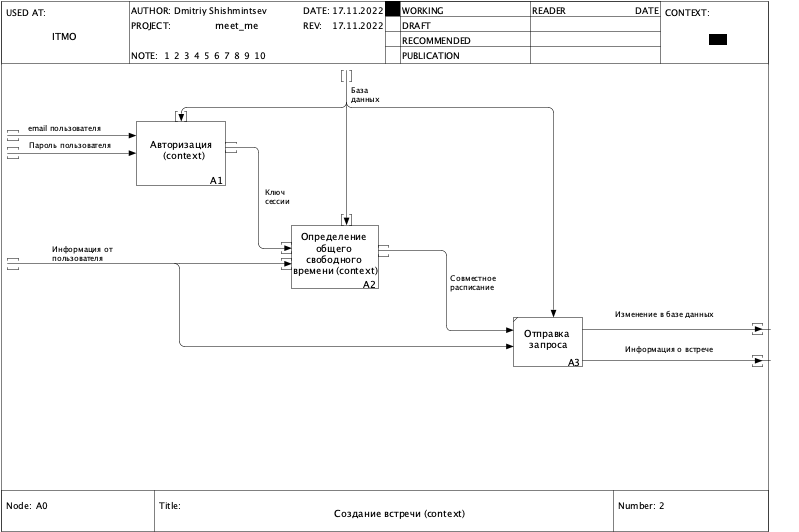
\includegraphics[width=0.9\linewidth]{img/IDEF0-1.png}
                \caption{ Декомпозиция контекстной диаграммы по стандарту IDEF0}
                \label{fig:d2}
            \end{figure}

            \begin{figure}[h]   
                \centering
                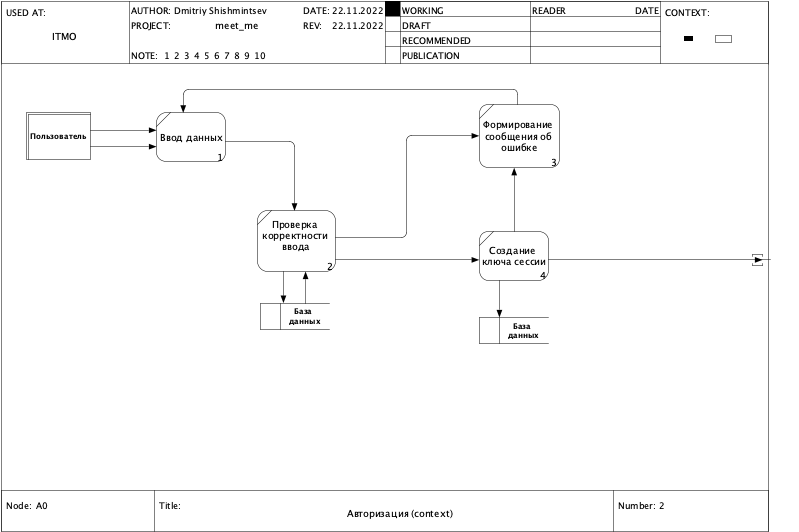
\includegraphics[width=0.9\linewidth]{img/DFD1.png}
                \caption{ Декомпозиция блока <<Авторизация>> по стандарту DFD}
                \label{fig:d3}
            \end{figure}

            \begin{figure}[h]   
                \centering
                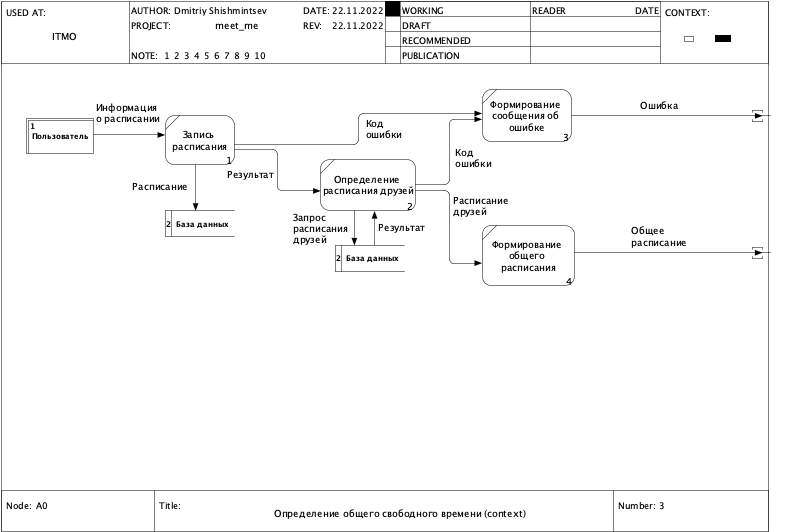
\includegraphics[width=0.9\linewidth]{img/DFD2.png}
                \caption{ Декомпозиция блока <<Определение общего свободного времени>> по стандарту DFD}
                \label{fig:d4}
            \end{figure}
        \end{landscape}

    \section{Модели по стандарту IDEF3}
        В данном разделе представлена контекстная диаграмма (рисунок \ref{fig:d5}), декомпозиция контекстой диаграммы (рисунок \ref{fig:d6}), декомпозиция блока <<Вход>> (рисунок \ref{fig:d7}), а так же декомпозиция блока <<Определение общего расписания>> (рисунок \ref{fig:d8}) согласно стандарту IDEF3. 
        \begin{landscape}
            \begin{figure}[h]   
                \centering
                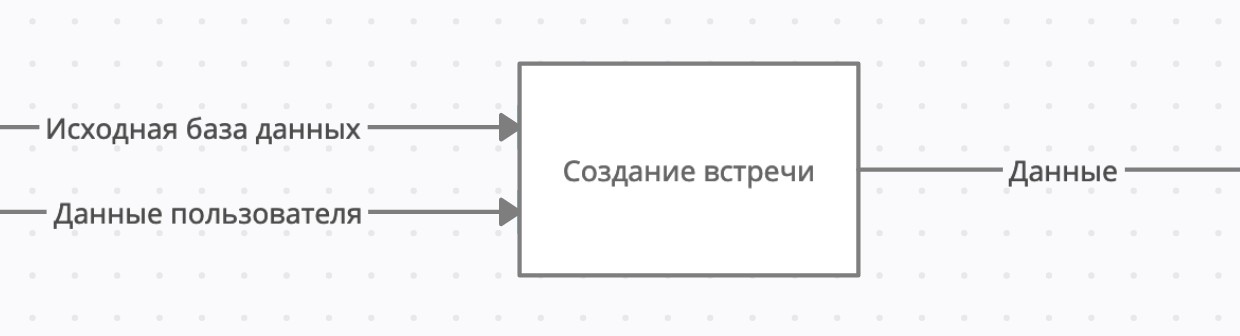
\includegraphics[width=0.7\linewidth]{img/IDEF3-0.png}
                \caption{ Контекстная диаграмма по стандарту IDEF3}
                \label{fig:d5}
            \end{figure}

            \begin{figure}[h]   
                \centering
                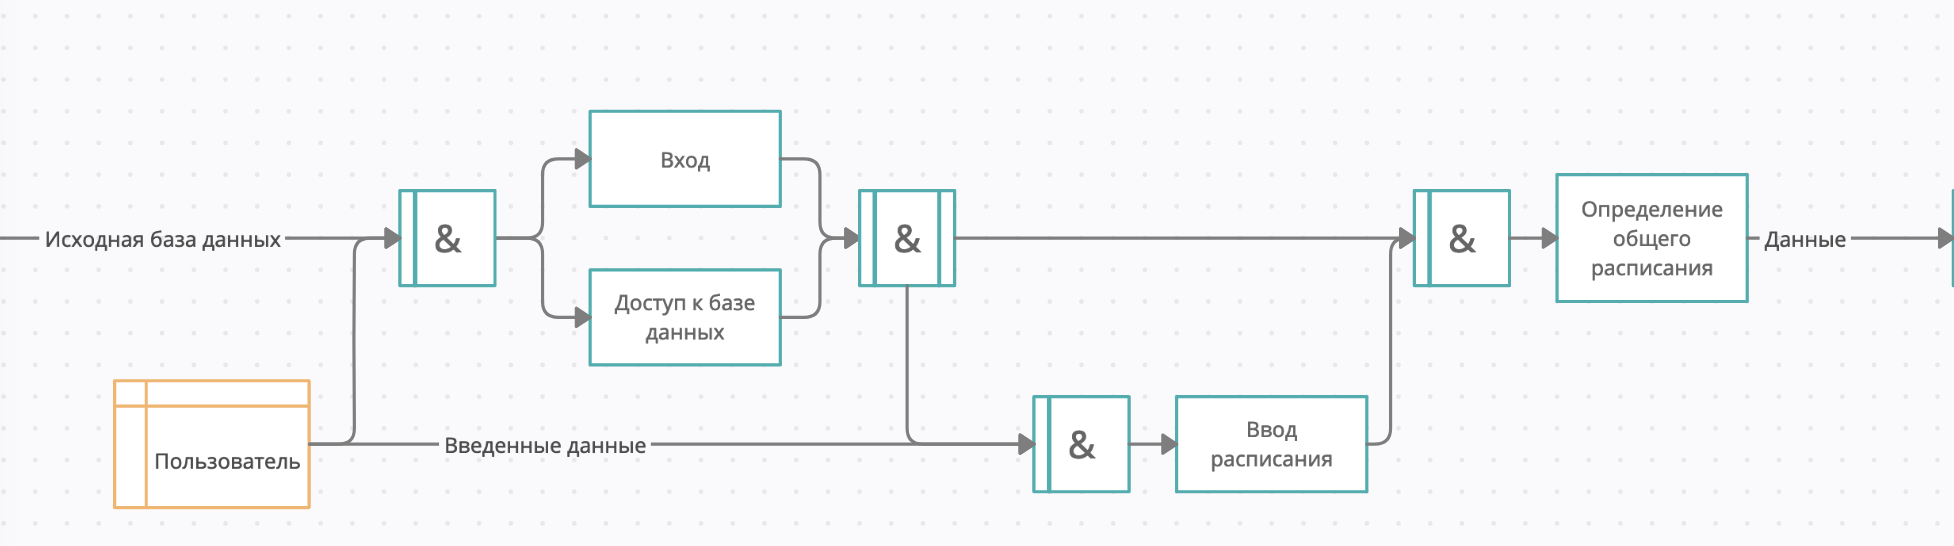
\includegraphics[width=0.7\linewidth]{img/IDEF3-1-0.png}
                \caption{ Декомпозиция контекстной диаграммы по стандарту IDEF3}
                \label{fig:d6}
            \end{figure}

            \begin{figure}[h]   
                \centering
                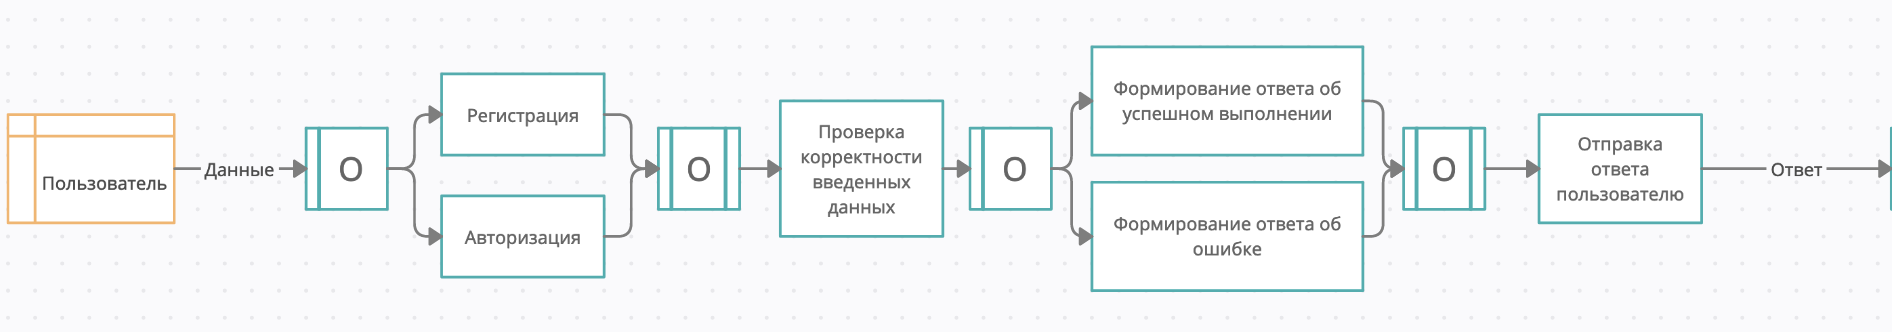
\includegraphics[width=0.9\linewidth]{img/IDEF3-2-0.png}
                \caption{ Декомпозиция блока <<Вход>> по стандарту IDEF3}
                \label{fig:d7}
            \end{figure}

            \begin{figure}[h]   
                \centering
                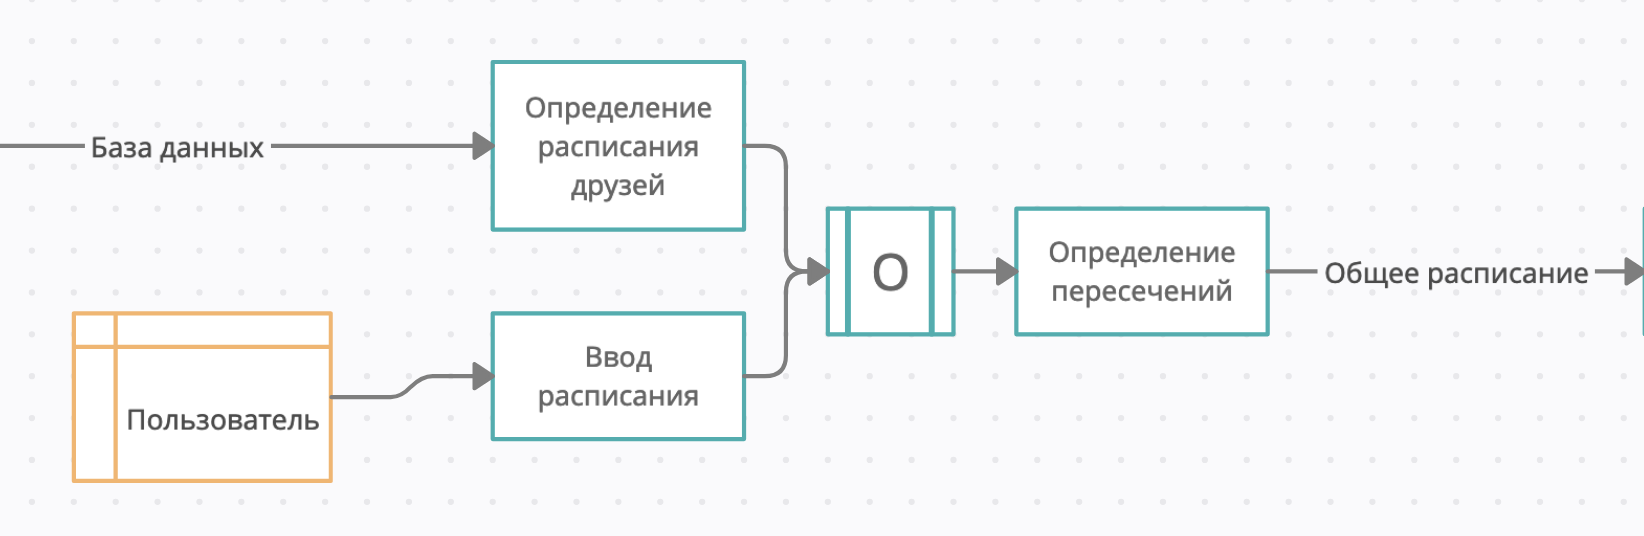
\includegraphics[width=0.9\linewidth]{img/IDEF3-2-1.png}
                \caption{ Декомпозиция блока <<Определение общего расписания>> по стандарту IDEF3}
                \label{fig:d8}
            \end{figure}
        \end{landscape}

    \section{Модель процесса в нотации BPMN}
        В данном разделе представлена модель процесса в нотации BPMN (рисунок \ref{fig:d9})
        \begin{figure}[h]   
            \centering
            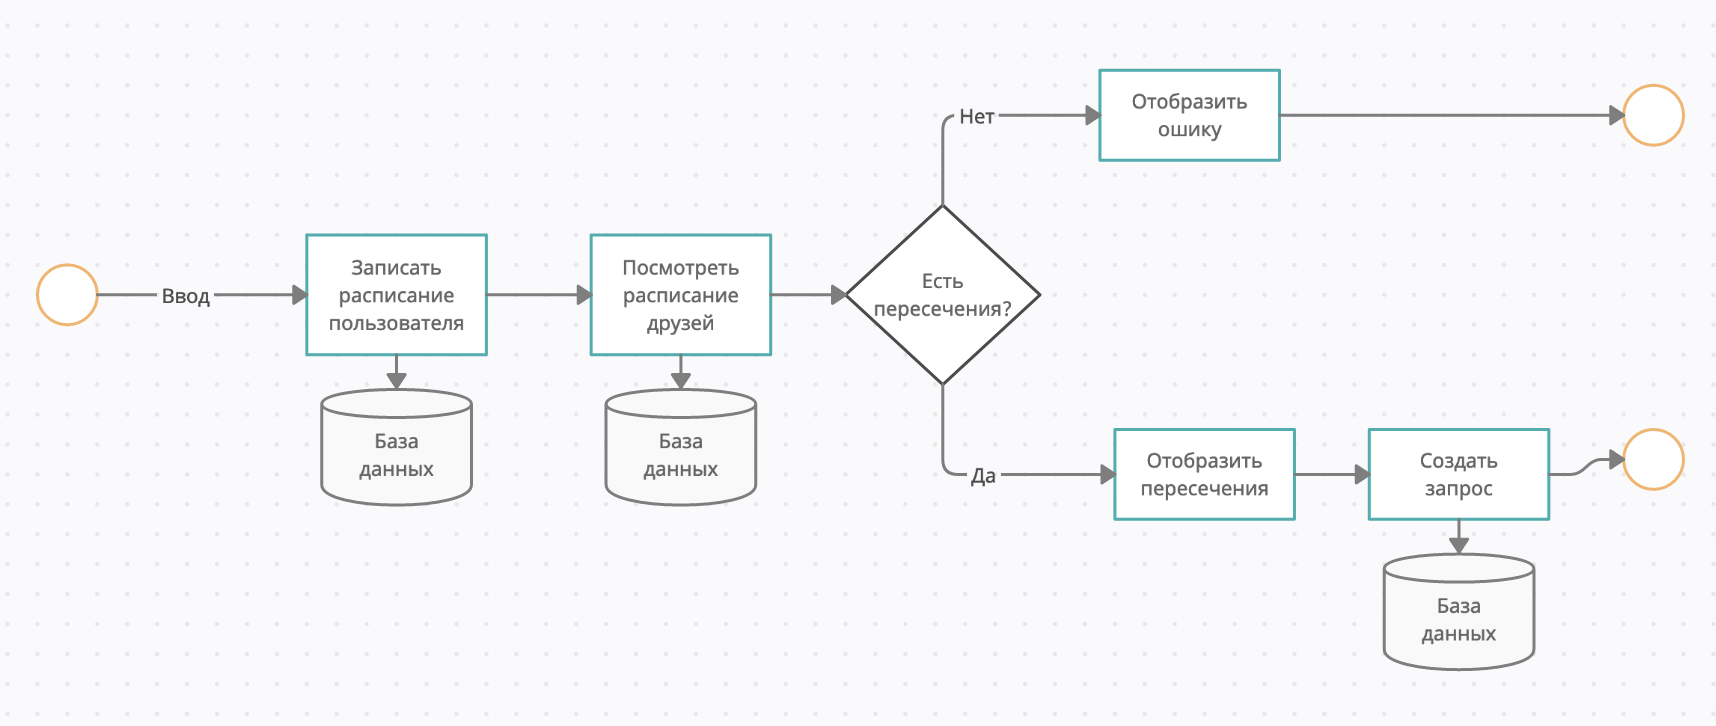
\includegraphics[width=0.9\linewidth]{img/BPMN.png}
            \caption{ Модель по стандарту BPMN}
            \label{fig:d9}
        \end{figure}

\conclusions

Был составлен отчет, кратко описана основная предметная область функционирования будующей информационной системы, разработаны модели по стандарту DFD в дополнение к моделям IDEF0, разработаны модели IDEF3 с несколькими уровнями декомпозиции, а так же модель процесса по стандарту BPMN.

\newpage
\begin{thebibliography}{99}
	\bibitem{bib1} 	\label{bib:bib1} В. И. Горбаченко. <<СОЗДАНИЕ ФУНКЦИОНАЛЬНОЙ МОДЕЛИ ИНФОРМАЦИОННОЙ СИСТЕМЫ С ПОМОЩЬЮ CASE-средства CA ERwin Process Modeler 7.3>> - Пенза 2010 - 25-55с.
\end{thebibliography}

\end{document}
